\newcommand*{\bx}{\bm{x}}
\newcommand*{\bX}{\bm{X}}
\newcommand*{\bxi}{\bm{x}_i}
\newcommand*{\delx}{\bx - \bxi}
\newcommand*{\by}{\bm{y}}
\newcommand*{\byi}{\bm{y}_i}
\newcommand*{\dely}{\by - \byi}
\newcommand*{\zbx}{Z(\bx)}
\newcommand*{\zbxi}{Z(\bxi)}
\newcommand*{\bb}{\bm{\beta}}
\newcommand*{\hzbx}{\hat{Z}(\bx)}
%
\subsection{Registration}
\begin{figure}
    \centering
    \begin{adjustbox}{width=\linewidth}
        \forestset{
          direction switch/.style={
            where level>=1{folder, grow'=0}{for children=forked edge},
          },
        }
        \begin{forest}
          direction switch
          [SR
            [MISR
              [Adapative Filtering]
              [Statistical
                [Back Projection]
                [Markov Random Fields]
                [Bilateral Total Variation]
              ]
            ]
            [SISR
                [Manifold Learning]
                [Compressed Sensing]
                [Projection]
                [Belief Networks]
            ]
          ]
        \end{forest}
    \end{adjustbox}
    \caption{Taxonomy of classical SR techniques}
    \label{fig:taxonomy}
\end{figure}

Figure~\ref{fig:taxonomy} lays out a rough taxonomy of classical SR algorithms.
%
We cover algorithms from each "genus" and others that don't neatly fit into the taxonomy.
\subsection{Interpolation}
Suppose that $H_k$ is linear spatial\anote{lsi} and time invariant.
%
Suppose further that $A_k$ is affine.
%
Then $H \coloneqq H_k$ commutes with $A_k$\cite{meladcommute} and eqn.~\ref{eqn:commuteimagingmodel} becomes
\begin{equation}
    \label{eqn:commuteimagingmodel}
    \begin{split}
        X_k &= (D \circ A_k \circ H) (Y) + \varepsilon \\
        &= (D \circ A_k) (H(Y)) + \varepsilon \\
        &= (D \circ A_k) (V) + \varepsilon
    \end{split}
\end{equation}
%
where $V \coloneqq H(Y)$.
%
This naturally suggests interpolation in order to recover $V$ (since $X_k$, in this framing, is simply shifted samples of $V$).
%
Note in this context we use interpolation very broadly, i.e. to connote filling in missing values using neighboring (in some sense --- not necessarily geometrically) values.
%
\begin{figure}
    \centering
    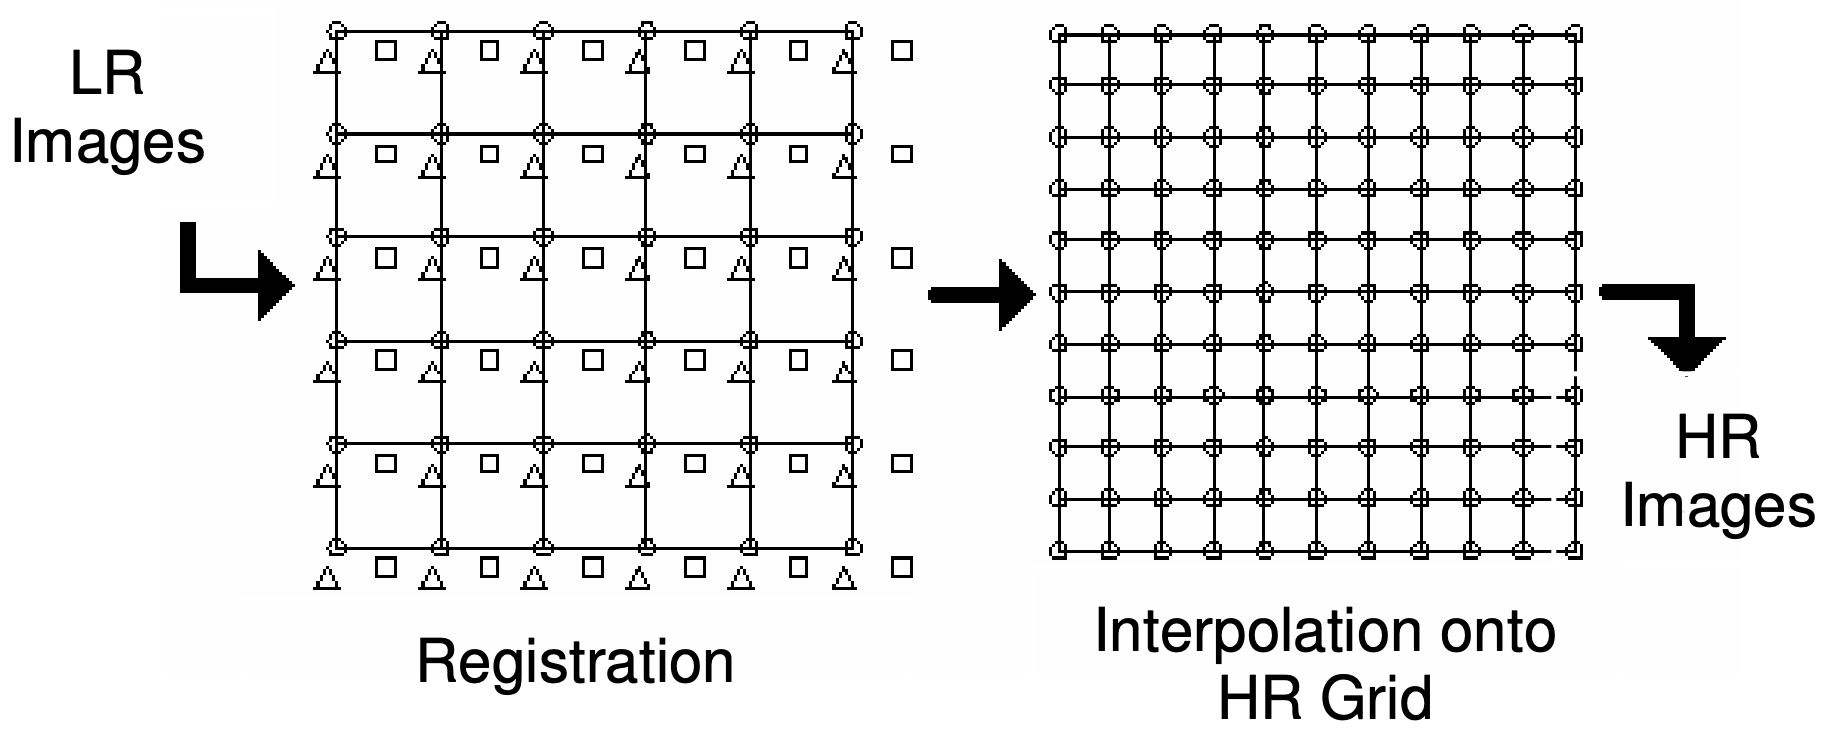
\includegraphics[width=\linewidth]{figures/hrgrid.png}
    \caption{LR image registration on an HR grid\cite{Lin}}
    \label{fig:hrgrid}
\end{figure}
This class of techniques proceed by first registering images on a high resolution grid (see figure~\ref{fig:hrgrid}) then interpolating at the "missing" pixels in the HR grid to recover $V$, and finally denoising and deconvolution (of $H$) to recover $Y$.
%
Since in general consecutive $X_k$ have non-uniform shifts (relative to $X_1$) the interpolation is non-uniform and improvisations on this theme use various weighting schemes for adjacent LR pixels\anote{lrpixel}.

For example Alam et. al\cite{Alam2000} uses weighted nearest neighbors: for every pixel to be interpolated the three nearest pixels are weighted inversely by their distance (according to HR grid distance) and then their weighted sum is assigned to that pixel.
%
This non-uniform interpolation is then followed by application of a Wiener filter whose design is informed by the OTF of the particular imaging system they study (which they do not estimate i.e. they assume they can model accurately).
%
\begin{figure}
    \centering
    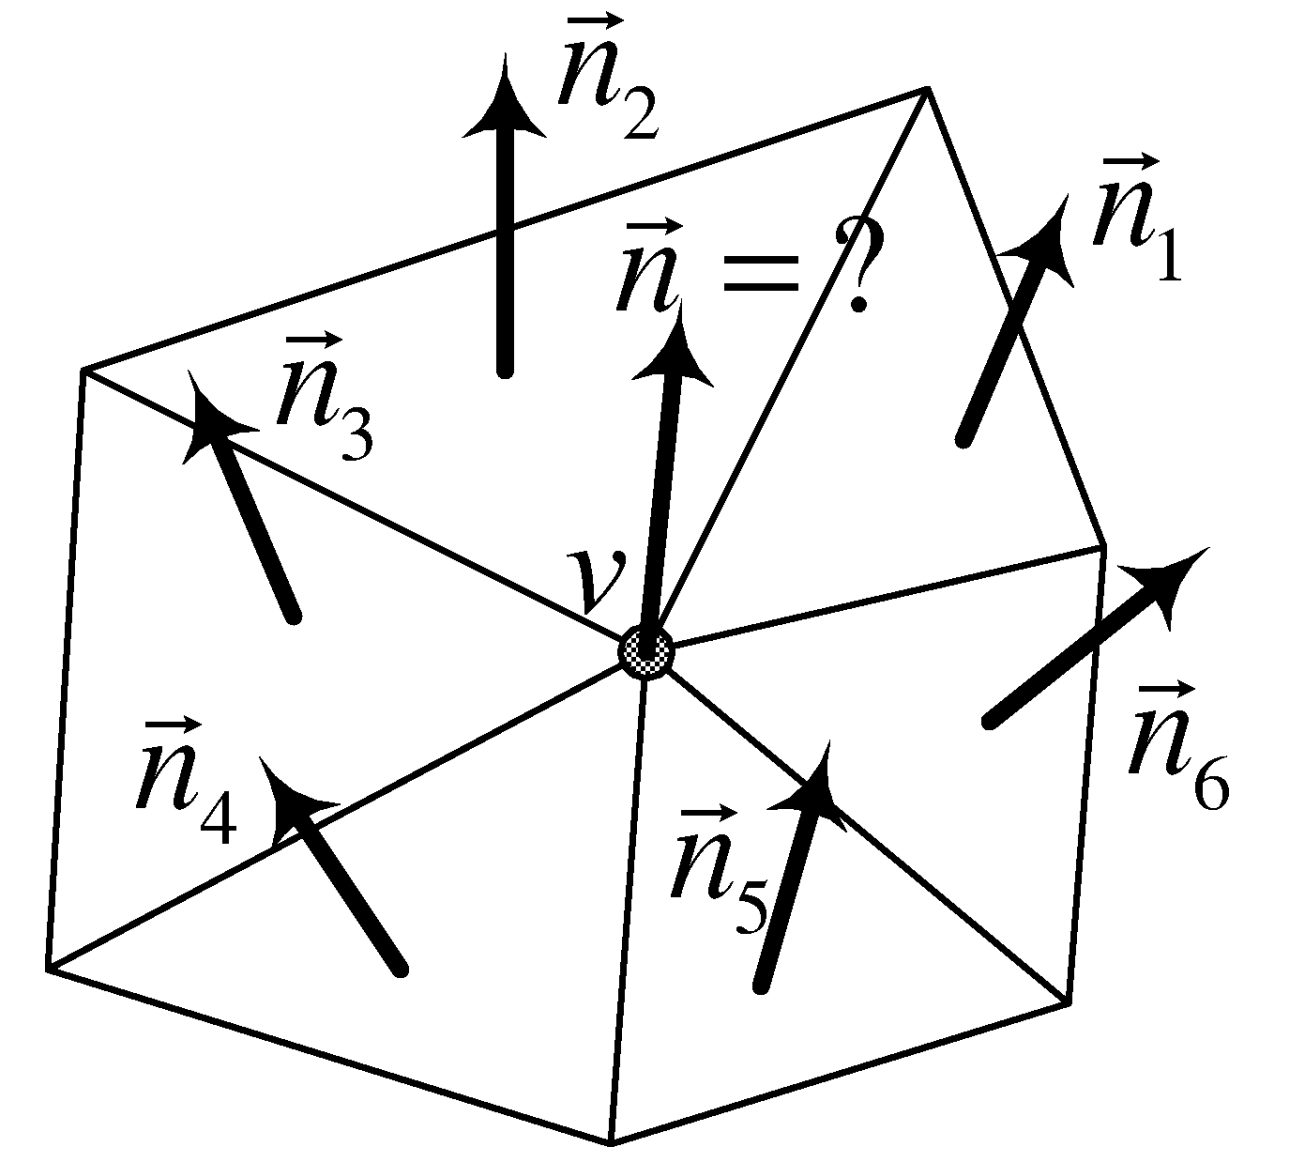
\includegraphics[width=.7\linewidth]{figures/delauney.png}
    \caption{Delaunay triangulation for fitting splines at LR pixels\cite{Lertrattanapanich}. $v$ is an LR pixel. Note that $v$ is at $z$ equal to the pixel value}
    \label{fig:delauney}
\end{figure}
Lertrattanapanich et. al\cite{Lertrattanapanich} base their algorithm on interpolants which require knowledge of gradients (e.g. splines) and mediate the non-uniform sampling by using a weighted average (by area) of those gradients in adjacent Delaunay cells; to be precise they produce a Delaunay triangulation of all LR pixels and compute the gradients (see figure~\ref{fig:delauney}) according to
\begin{align*}
    \vec{n} = \sum_{i=1}^m \frac{B_j \vec{n_j}}{B} &\text{ where } B=\sum_{i=1}^m B_i\\
    \frac{\partial z}{\partial x} = -\frac{n_x}{n_z} &\text{ and }  \frac{\partial z}{\partial y} = -\frac{n_y}{n_z}
\end{align*}
where $B_i$ is the area of the $i$th Delaunay cell.
%
Unfortunately this intricate solution is not robust to noise in real images.

A more sophisticated method for non-uniform interpolation uses parametric models for the auto-correlation between LR pixels and the cross-correlation between LR pixels and interpolated pixels to estimate wiener filter weights\cite{wiener}.
%
These weights are then used to average nearby pixel values.
%
The algorithm operates on a sliding \textit{estimation window} whose dimensions $D_x, D_y$ are chosen such that the effective sampling rate exceeds the Nyquist rate for a given $\rho_c$.
\begin{figure}
    \centering
    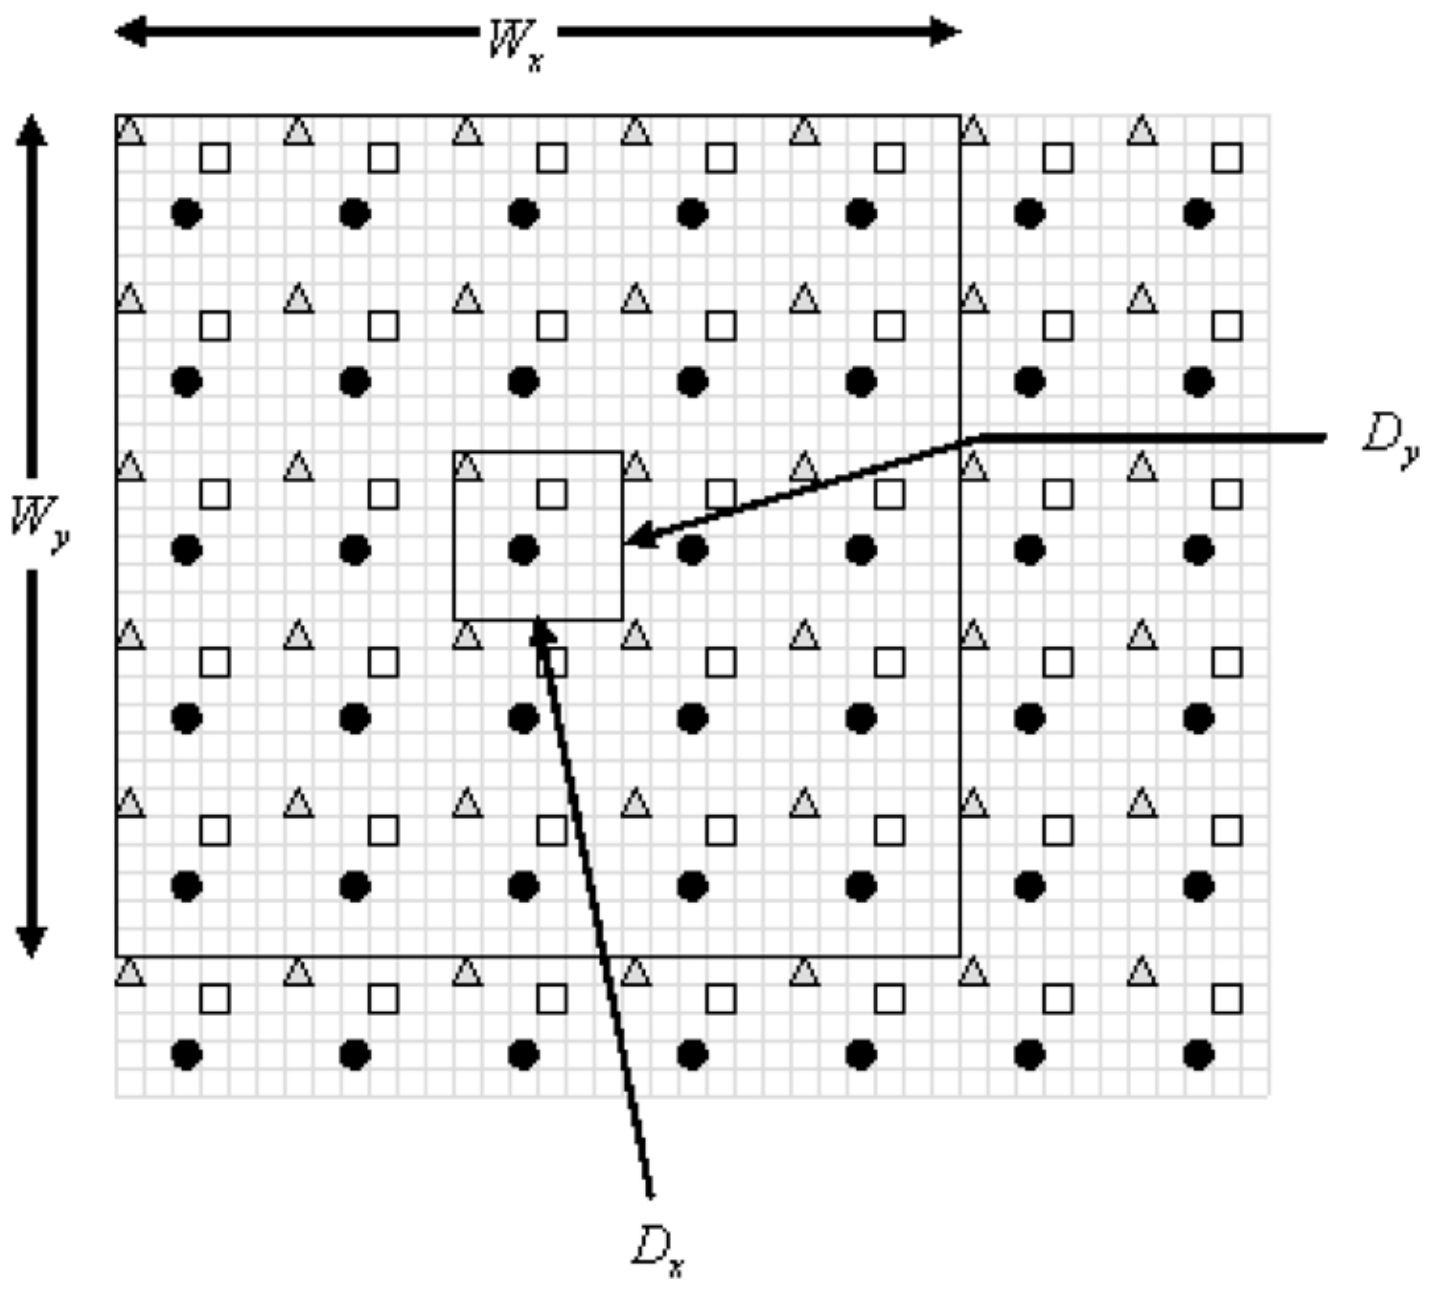
\includegraphics[width=.7\linewidth]{figures/wiener.png}
    \caption{Wiener filter super resolution estimation window of dimension $D_x \times D_y$ and observation window of dimension $W_x \times W_y$\cite{wiener}}
    \label{fig:wiener}
\end{figure}
The pixel values for the estimation window are a function of the wiener filter weights of nearby LR pixels within an \textit{observation window} whose dimensions $W_x, W_y$ are an integer multiple of $D_x, D_y$ (see figure~\ref{fig:wiener}).
%
The weights $\bm{w}$ are defined as the solution to the minimum mean squared error (MMSE) filter problem, i.e. the finite impulse response (FIR) wiener filter:
\begin{equation}
    \bm{w} = R^{-1}\bm{p}
\end{equation}
where $R$ is the auto-correlation of the LR pixels in the observation window and $\bm{p}$ is the cross-correlation between the pixels to be estimated and the LR pixels.
%
Then $R$ and $\bm{p}$ are both constructed by sampling a parametric model that weights pixels in the observation window according to distance:
%
$R$ is constructed by sampling from
\begin{equation}
    C_1(r) \coloneqq \sigma_{d}^2 \rho^{r} \ast G(r)
\end{equation}
and $\bm{p}$ is constructed by sampling from
\begin{equation}
    C_2(r) \coloneqq \sigma_d^2 \rho^{r} \ast G(r) \ast G(-r)
\end{equation}
In the case of $R$, $r$ is distance on the HR grid, $\sigma_d$ is related to the empirical variance of all LR pixels in a given observation window and $G(r)$ is a smoothing kernel (e.g. Gaussian).
%
Thus by evaluating $C_1$ for all $r = r(n_1, n_2)$ distances between LR pixels $n_1$, $n_2$ we can construct $R$.
%
Similarly for $\bm{p}$, $r = r(m, n)$ is the distance between pixel-to-be-estimated $m$ and LR pixel $n$.
%
Note that $R$ is an $N \times N$ matrix where $N = K W_x W_y/D_x D_y$, i.e. how many LR pixels there are in the observation window, and $\bm{p}$ is an $N \times 1$ column vector uniquely computed for each pixel in the estimation window.
%
The scheme is effective but suffers from issues with the spatial isotropy of the auto-correlation and cross-correlation models.

One of the most sophisticated of these non-uniform interpolation schemes employs the kernel regression framework and \textit{steering kernels}\cite{Takeda2007}.
%
In this context we start with all $X_k$ registered to a common HR grid and consider pixel values $Y(\bxi)$ at pixel coordinates $\bxi \coloneqq (x_{i1},x_{i2})$ as the measured data pairs $(\bxi, Y(\bxi)$.
%
Recall that kernel regression frames the estimation problem as
\begin{equation}
    Y(\bxi) = Z(\bxi) + \varepsilon
\end{equation}
where $Z$ is the to-be-estimated \textit{regression function} that "predicts" $Y$ as a function of $\bx$.
Then the Nadaraya–Watson estimator (NWE)\cite{Nadaraya} $\hat{Z}$ for $Z$ is
\begin{equation}
    \hat{Z}(\bx) = \frac{\sum_{i=1}^{P}K(\delx)Y(\bxi)}{\sum_{i=1}^{P}K(\delx)}
    \label{eqn:kernelregression}
\end{equation}
where $P$ indexes over all pixels in the HR grid and $K$ is a \textit{kernel function} whose purpose is to decay the contribution of $\bxi$ if it's in some sense far from $\bx$.
%
Note that $\hat{Z}(\bx)$ can also be seen as a weighted filtering of $Y$.
%
\begin{figure}
    \centering
    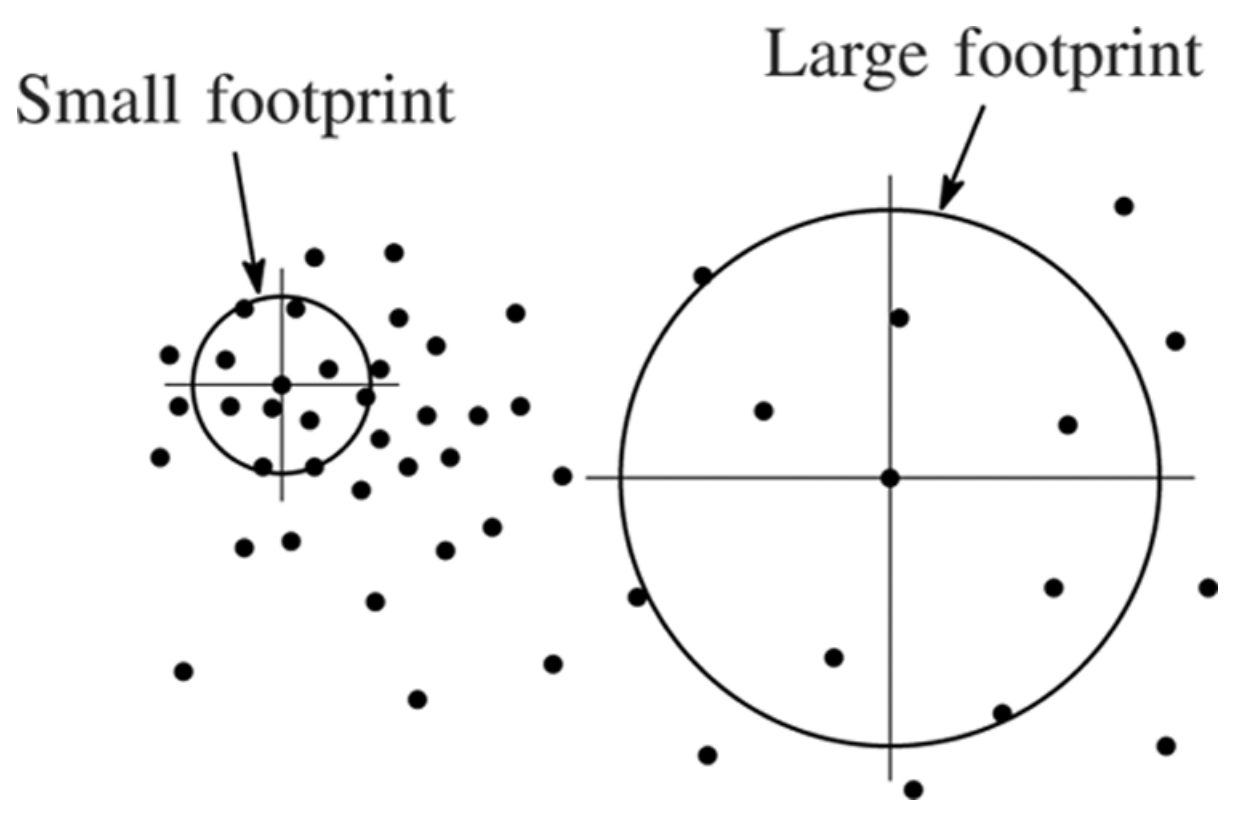
\includegraphics[width=.8\linewidth]{figures/footprint.png}
    \caption{Kernel footprint as a function of sample density\cite{Takeda2007}}
    \label{fig:footprint}
\end{figure}
\begin{figure}
    \centering
    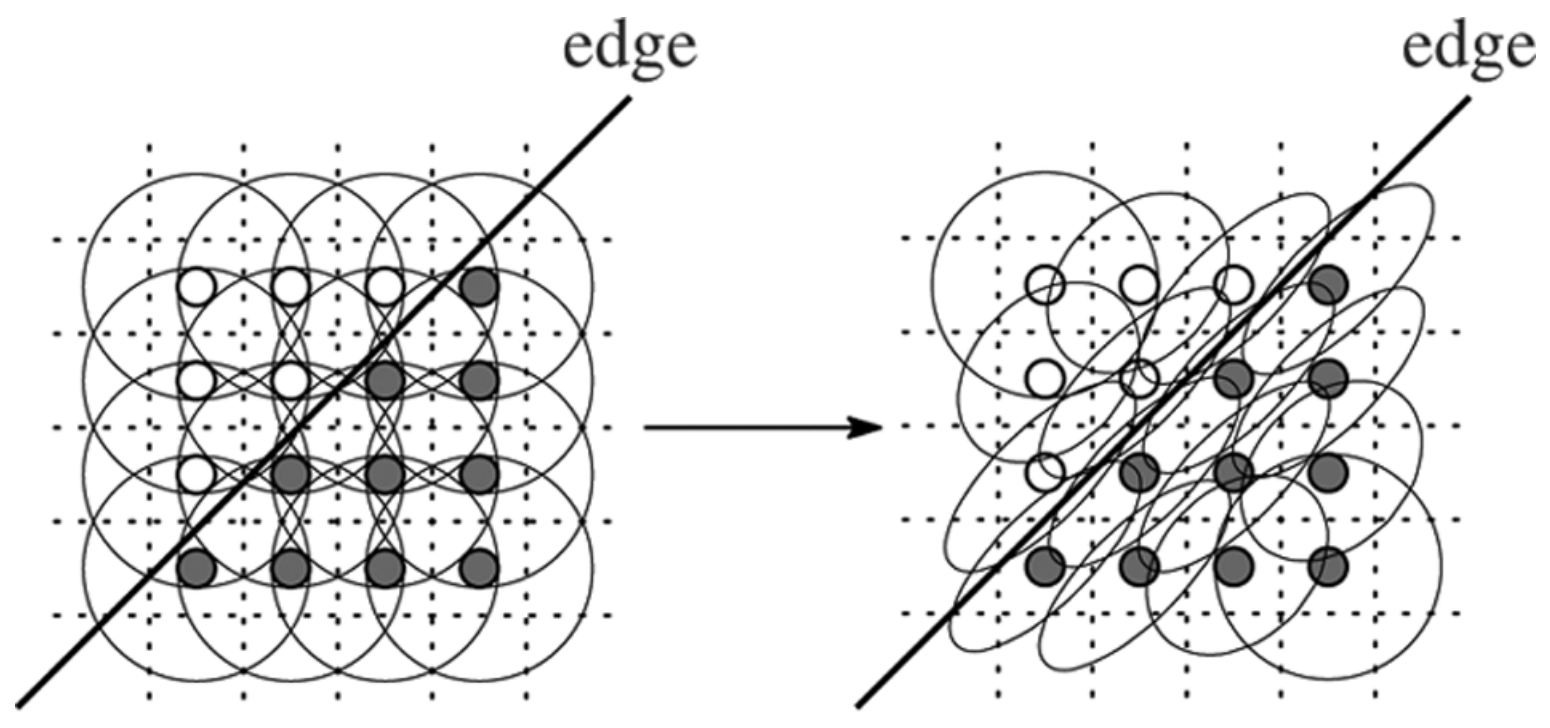
\includegraphics[width=\linewidth]{figures/steering.png}
    \caption{Adapting kernel shape as a function of local directed structure\cite{Takeda2007}}
    \label{fig:steering}
\end{figure}
In conventional kernel regression $K$ might be any non-negative, symmetric, unimodal\cite{wand1994kernel} function with augmented with an additional $h$ parameter that controls the "bandwidth" or "footprint" of the kernel, i.e.
\begin{equation}
    K_h(\delx) \coloneqq \frac{1}{h}K\left( h^{-1}(\delx) \right)
\end{equation}
This bandwidth parameter $h$ can be generalized to a \textit{smoothing kernel} $H$ in order to make $K = K_H$ adaptive to the local structure of the pixels, e.g. to have larger footprints in sparsely sampled regions and have smaller footprints in densely sampled regions (see figure~\ref{fig:footprint}).
%
Ultimately though it is desirable to have kernels that can adapt to directed structure in the image, i.e. "steerable" kernels that filter strongly along an edge and weakly across an edge.
%
This is accomplished by, for example, using a Gaussian as the kernel:
\begin{equation}
    K_{H_i}(\delx) \propto \frac{\exp\left\{ -(\delx)^T H^{-1}_i (\delx) \right\}}{\sqrt{\det{H_i}}}
\end{equation}
and identifying $H_i$ with $\nabla^2 \zbxi$ (since gradients capture edge structure).
%
An estimate $\hat{H}_i$ of $\nabla^2 \zbxi$ can be obtained by looking at covariances of empirical gradients (i.e. the HR grid registered image convolved with a difference filter).
%
Unfortunately this is a naive estimate that is often rank deficient or unstable (both leading to instances where $\hat{H}_i$ isn't invertible).
%
One solution is to parameterize $H_i$:
\[
    H_i = \gamma_i U_{\theta_i} \Lambda_{\sigma_i} U_{\theta_i}^T
\]
where $U_{\theta_i}$ is a rotation matrix, $\Lambda_{\sigma_i} = \text{diag}\left( \sigma_i, \sigma_i^{-1} \right)$ is an "elongation" matrix, and $\gamma_i$ is a scaling parameter, with each of $\gamma_i, \theta_i, \sigma_i$ estimated from the data in a more robust way.
%
An alternative kernel is the bilateral kernel\cite{Tomasi:1998:BFG:938978.939190} that defines closeness according to geometric and radiometric distance:
\begin{equation}
    \begin{split}
        K_S(\delx) &\coloneqq \exp \left\{ \frac{\left\| \delx \right\|^2}{2 \sigma_S^2}  \right\} \\
        K_R(\delx) &\coloneqq \exp \left\{  \frac{\left\| Y(\bx) - Y(\bxi) \right\|^2}{2 \sigma_R^2} \right\} \\
        K_B(\delx) &\coloneqq K_S(\delx)K_R(\delx)
    \end{split}
    \label{eqn:bilateralkernel}
\end{equation}
where $\sigma_S$ parameterizes spatial distance weight and $\sigma_R$ parameterizes "radiometric" distance weight.

In general non-uniform interpolation techniques are intuitive and typically (relatively) computationally efficient but they assume an unrealistic observation model (namely that of affine flow).

\subsection{Estimation}

Statistical estimation methods cast SR as an inference problem.
%
One of the earliest successful SR algorithms\cite{Irani1991ImprovingRB} proposed an iterative scheme inspired by the back-projection method commonly used to reconstruct 2-D objects from 1-D projections in computer-aided tomography.
%
Recall eqn.~\ref{eqn:imagingmodel}.
%
Then the idea is to take the current estimate of the HR image $\hat{Y}^{i}$, see if after motion and down-sampling $(D \circ A_k)(\hat{Y}^i)$ it is near the LR samples $X_k$, and add a correction when it is not:
\begin{equation}
    \hat{Y}^{i+1} = \hat{Y}^i + \sum_{k=1}^K (D \circ A_k)^{-1}\left( (D \circ A_k)(\hat{Y}^i) - X_k \right)
    \label{eqn:ibp}
\end{equation}
where $\hat{Y}^i$ is the current estimate of the blurred HR image, $(D \circ A_k)(\hat{Y}^i)$ is the projection of the current estimate to low resolution, and $(D \circ A_k)^{-1}\left( (D \circ A_k)(\hat{Y}^i) - X_k \right)$ is the \textit{back-projection}.
%
This process iterates until convergence i.e. $\lvert (D \circ A_k)(\hat{Y}^i) - X_k \rvert < \delta$ for some $\delta$.
%
Irani et al.\cite{Irani1991ImprovingRB} also convolve the back-projection with a smoothing kernel as a form of regularization since the estimation problem is in general ill-posed (there are many $\hat{Y}^{i}$ that will project down to a pixel-distance neighbor of $X_k$).
%
It can be shown\cite{Elad1996} that for $\varepsilon_k$ distributed $(0, R_k)$-Normal, $\hat{Y}$ is none other than the maximum likelihood estimate (MLE) for $Y$.
%
We can see this by recognizing that eqn.~\ref{eqn:ibp} is just the Richardson iterative\cite{Anderssen:1972:RNM:891962} solution to
\begin{equation}
    L(Y) = \frac{1}{2} \left\| \bm{X} -  \begin{bmatrix}
                                             D_1 \circ A_1 \\
                                             D_2 \circ A_2 \\
                                             \vdots \\
                                             D_K \circ A_K \\
    \end{bmatrix}  Y  \right\|^2
    \label{eqn:l2regression}
\end{equation}
since
\begin{gather*}
    \nabla_{Y} L = 0 \\
    \iff \\
    \sum_{k=1}^K (D \circ A_k)^{-1}\left( (D \circ A_k)(Y) - X_k \right) = 0
\end{gather*}
and therefore $\hat{Y}_i \rightarrow \hat{Y}$ is the MLE (since MLE is the solution to least squares\cite{CaseBerg:01}).
%
Though this is one of the oldest SR algorithms it's recently been revisited and re-imagined as a deep neural network architecture (DNN)\cite{DBLP:journals.corr.abs-1803-02735}.

Another estimation technique employs a Kalman filter\cite{elad1999} to estimate $Y$.
%
Let $\bm{x}_k = \text{vec}(X_k)$ be the vectorization\anote{vectorize} of $X_k$ and $\bm{y} = \text{vec}(Y)$ likewise.
%
If we assume linear models for each of $D, A_k, H_k$ (i.e. all representable as matrices) and a well-behaved optical flow model (most pixels in image $\bm{x}_k$ appear in image $\bm{x}_{k-1}$) then we can image $\bm{y}$ as a sequence of images $\bm{y}_k$ related in time by
\begin{equation}
    \bm{y}_k = A'_k \bm{y}_{k-1} + \eta_k
    \label{eqn:kalmanprocess}
\end{equation}
%
where $A'_k$ is the \textit{relative} motion operator, $A'_k\bm{y}_{k-1}$ is conventional matrix-vector multiplication, and $\eta_k$ is the only source of new pixels (noise\anote{noise} distributed $(0, Q_k)$-Normal).
%
Consequently eqn.~\ref{eqn:imagingmodel} becomes
\begin{equation}
    \bm{x}_k = DH_k\bm{y}_k + \varepsilon_k
    \label{eqn:kalmanobs}
\end{equation}
and the pair of eqns.~\ref{eqn:kalmanprocess},~\ref{eqn:kalmanobs} can be seen to constitute a linear dynamical system with $\bm{y}_k$ the state of the system, $A'_k$ the state transition, $\eta_k$ the state noise, $\bm{x}_k$ the measurement, $DH_k$ the measurement model, and $\varepsilon_k$ the measurement noise.
%
Note that the HR image conditioned on all previous LR images (measurements)
\begin{equation}
    \bm{y}_{k|s} \coloneqq \bm{y}_k|\bm{x}_1, \mathellipsis, \bm{x}_s
\end{equation}
with $s \leq k$, is a Gaussian process (GP), with mean $\bar{\bm{y}}_{k|s} = E\left[\bm{y}_{k|s}\right]$
and covariance
\begin{equation}
    C_{k|s} \coloneqq E\left[ (\bm{y}_k - \bar{\bm{y}}_{k|s})(\bm{y}_k - \bar{\bm{y}}_{k|s})^T  \right]
\end{equation}
%
By definition the MMSE $\hat{\bm{y}}_{k|s}$ of $\bm{y}_{k|s}$ is $\bar{\bm{y}}_{k|s}$ and therefore $C_{k|s}$ is the covariance of the error of the estimate $\hat{\bm{y}}_{k|s}$.
%
The Kalman filter proceeds in two steps: an \textit{a priori} (before measurement) prediction step and an \textit{a posteriori} (after measurement) update step.
%
The prediction step iterates on the estimate (and its covariance) given all previous measurements:
\begin{align}
    \hat{\bm{y}}_{k|k-1} &= A'_k \hat{\bm{y}}_{k-1|k-1} \\
    C_{k|k-1} &= A'_k C_{k-1|k-1} (A'_k)^T + Q_k
\end{align}
This can be seen as a one-step propagation of the estimate "in the direction" of the previous measurement.
%
Then the update step incorporates new information from a measurement:
\begin{align}
    \hat{\bm{y}}_{k|k} &= \hat{\bm{y}}_{k|k-1} + K_k(\bm{x}_k - DH_k\hat{\bm{y}}_{k|k-1} ) \\
    C_{k|k} &= (I - K_k DH_k)C_{k|k-1}
\end{align}
where the \text{Kalman gain}
\begin{equation}
    K_k \coloneqq \frac{C_{k|k-1}(DH_k)^T}{DH_k C_{k|k-1} (DH_k)^T + R_k }
\end{equation}
weights the contribution of the prediction and the measurement\anote{kalmanprediction}.
%
Note that in the Kalman framework $D, H_k, A'_k, R_k, Q_k$ are all assumed to be known.
%
In Elad et al.\cite{elad1999} the assumption is $D, H_k, R_k$ are known functions of camera parameters, $A'_k$ can be estimated by an image registration algorithm and $Q_k$ can be approximated:
\begin{equation}
    Q_k \approx \alpha_k A'_k C_{k|k} (A'_k)^T
\end{equation}
where $\alpha_k$ is chosen such that the approximation upper-bounds the true $Q_k$.
%
They comment that this stronger auto-correlation for $\bm{y}_k$ adds "pseudo-noise" to the system and biases the Kalman filter to "rely" more on the measurements than the state transition model.

SR can also be posed as a Bayesian maximum a posterior (MAP) estimation problem.
%
Let $\bm{H} \coloneqq \left( H_1, \mathellipsis, H_k \right)$ be the vector of blur operators applied to $Y$ in order to produce $\bm{X}$ and similarly $\bm{A}$ then
\begin{align}
    \hat{Y} &= \underset{Y}{\text{argmax}}~P\left( Y | \bm{X} \right) \nonumber \\
    &= \underset{Y}{\text{argmax}} \int_{D, \bm{H}, \bm{A}} P\left( Y, D, \bm{H}, \bm{A} | \bm{X}\right) \nonumber \\
    &= \underset{Y}{\text{argmax}} \int_{D, \bm{H}, \bm{A}} \frac{P\left(\bm{X} | Y, D, \bm{H}, \bm{A} \right)P(Y) P(D, \bm{H}, \bm{A})}{P(\bm{X})}\label{eqn:indepym} \\
    \hat{Y} &= \underset{Y}{\text{argmax}} \int_{D, \bm{H}, \bm{A}} P\left(\bm{X} | Y, D, \bm{H}, \bm{A} \right)P(Y) P(D, \bm{H}, \bm{A}) \label{eqn:maxx}
\end{align}
where in eqn.~\ref{eqn:indepym} we've used the independence of $Y$ and $D, \bm{H}, \bm{A}$\cite{Hardie1997} and in eqn.~\ref{eqn:maxx} we've used that $\bm{X}$ is a constant with respect to the maximization.
%
While there exist reasonable priors for $Y$, marginalizing over $D, \bm{H}, \bm{A}$ is still difficult due to the high-dimensionality of each.
%
Therefore assuming $D, \bm{H}, \bm{A}$ can be estimated independently as $\hat{D}, \hat{\bm{H}}, \hat{\bm{A}}$, eqn.~\ref{eqn:maxx} becomes
\begin{equation}
    \hat{Y} = \underset{Y}{\text{argmax}}~P\left(\bm{X} | Y; \hat{D}, \hat{\bm{H}}, \hat{\bm{A}} \right) P(Y)
    \label{eqn:map}
\end{equation}
where the semicolon indicates $\hat{D}, \hat{\bm{H}}, \hat{\bm{A}}$ are known parameters of the conditional distribution.
%
This casts $\hat{Y}$ the standard MAP estimate of $Y$.
%
Note that an equivalent formulation of MAP maximizes the log-likelihood instead of maximizing the likelihood:
\begin{align}
    \hat{Y} &= \underset{Y}{\text{argmax}}~P\left(\bm{X} | Y; \hat{D},  \hat{\bm{H}}, \hat{\bm{A}}\right) P(Y) \nonumber \\
    &=  \underset{Y}{\text{argmax}}\left[ \log{P\left(\bm{X} | Y; \hat{D},  \hat{\bm{H}}, \hat{\bm{A}} \right)} + \log{P(Y)} \right]
    \label{eqn:logmap}
\end{align}
%
Various choices for $P\left(\bm{X} | Y; \hat{D},  \hat{\bm{H}}, \hat{\bm{A}} \right)$ and the prior $P(Y)$ (and consequent choice of optimization strategies) characterize this class of SR techniques.
%
Again assume $D, H_k, A_k$ linear and given $\varepsilon_k$ in eqn.~\ref{eqn:imagingmodel} distributed $(0, rI)$-Normal
\begin{equation}
    P\left(\bm{X} | Y; \hat{D},  \hat{\bm{H}}, \hat{\bm{A}} \right) \propto \exp \left\{ -\frac{\left\| \bm{X} - \hat{D} \hat{\bm{H}} \hat{\bm{A}} \bm{y} \right\|^2}{2r^2} \right\}
\end{equation}
where here $\bm{X} = \left( \text{vec}(X_1), \mathellipsis, \text{vec}(X_k) \right)$ and
\begin{equation}
    \hat{D} \hat{\bm{H}} \hat{\bm{A}} \coloneqq \begin{bmatrix}
                                                    \hat{D} \hat{\bm{H}}_1 \hat{\bm{A}}_1 \\
                                                    \hat{D} \hat{\bm{H}}_2 \hat{\bm{A}}_2 \\
                                                    \vdots \\
                                                    \hat{D} \hat{\bm{H}}_K \hat{\bm{A}}_K \\
    \end{bmatrix}
\end{equation}
%
After a suitable choice for the prior it can be seen that eqn.~\ref{eqn:logmap} is just regularized regression.
%
For example when choosing a Gibbs\cite{Hardie1997} distribution as the prior, i.e.
\begin{equation}
    P(Y) \propto e^{-\alpha B(Y)}
    \label{eqn:gibbs}
\end{equation}
where $B(Y)$ is called the \textit{potential}, eqn.~\ref{eqn:logmap} becomes
\begin{equation}
    \hat{\bm{y}} = \underset{\bm{y}}{\text{argmin}}\left[ \left\| \bm{X} - \hat{D} \hat{\bm{H}} \hat{\bm{A}} \bm{y} \right\|^2 +\lambda B(Y)\right]
    \label{eqn:minmap}
\end{equation}
where the aggregate regularization parameter $\lambda$ absorbs $\alpha$ from $P(Y)$ and $r$ from $\varepsilon_k$.
%
There are many other choices for the prior in eqn.~\ref{eqn:logmap}, whose effect is to bias the estimator $\hat{\bm{y}}$ towards "natural" images.
%
Alternatively we can (and will) take eqn.~\ref{eqn:minmap} as our starting point and explicitly choose the regularizer $B(Y)$.

One of the simplest priors is a $(0, Q)$-Normal, where $Q$ is symmetric positive definite\anote{positivedef} (PD) and captures the covariance.
%
This corresponds to the regularizer taking the form
\begin{equation}
    B(Y) = \by ^T Q \by
\end{equation}
where $\by = \text{vec}(Y)$.
%
Since $Q$ is symmetric PD eqn.~\ref{eqn:minmap} becomes
\begin{equation}
    \hat{\bm{y}} = \underset{\bm{y}}{\text{argmin}}\left[ \left\| \bm{X} - \hat{D} \hat{\bm{H}} \hat{\bm{A}} \bm{y} \right\|^2 +\lambda \left\| \sqrt{Q}\bm{y} \right\|^2 \right]
    \label{eqn:tikminmap}
\end{equation}
where $\sqrt{Q}$ is $U$ of the Cholesky decomposition $Q = U^T U$.
%
Equation~\ref{eqn:tikminmap} is Tikhonov regularized regression.
%
Letting $G = \hat{D} \hat{\bm{H}} \hat{\bm{A}}$ the closed-form solution to eqn.~\ref{eqn:tikminmap} is
\begin{equation}
    \hat{\by} = \left( G^T G + \lambda Q \right)^{-1} G^T\bX
    \label{eqn:closedform}
\end{equation}
Nguyen et al.\cite{milanfar2001} use cross-validation to determine the regularization parameter $\lambda$ (by partitioning the pixels into a "fit" and "validate" set).
%
In general, rather than explicitly computing inverses in eqn.~\ref{eqn:closedform}, in practice $\hat{\bm{y}}$ is found by solving the regression problem via optimization (for high-dimensional matrices optimization is faster than inversion).
%
Nguyen et al. use conjugate gradient descent\anote{conjugategradients} to optimize eqn.~\ref{eqn:tikminmap}.
%
They argue that $\hat{D} \hat{\bm{H}} \hat{\bm{A}}$ is ill-conditioned\anote{illcondition} and to that end, since the convergence rate of conjugate gradients is dependent on the condition number\cite{vanderSluis1986}, propose pre-conditioners\anote{precondition} to improve the converge rate.

An issue with the multivariate Normal prior is that it strongly enforces global smoothness, penalizing sharp edges.
%
One solution is to use Huber loss\cite{huber1964}
\begin{equation}
    L_{\delta }(a)\coloneqq {
    \begin{cases}
        a^2 & \text{for }\lvert a \rvert \leq \delta \\
        2 \delta \lvert a \rvert - \delta^2 &{\text{otherwise}}
    \end{cases}
    }
\end{equation}
to explicitly parameterize the penalty for gradients (i.e. high-frequency features).
%
Huber loss enforces local smoothness (since it's quadratic for $\lvert a \rvert \leq \delta$) but permits edges (since it's linear for $\lvert a \rvert > \delta$).
%
Capel et al.\cite{capel2000} implement this by composing $L_{\delta }(a)$ with a first-order gradient operator\anote{gradientoperator} as the potential in eqn.~\ref{eqn:gibbs}.
%
Another gradient penalty that encourages sparse gradients (i.e. local smoothness and steep edges) is Total Variation (TV) norm\cite{RUDIN1992259}:
\begin{equation}
    \|u\|_{\operatorname {TV}}\,\coloneqq\int _{\Omega }\|\nabla u\|\,d\Omega
\end{equation}
where $u$ is a smooth image of bounded variation (i.e. such that the integral converges) over domain $\Omega$.
%
In the context of SR this amounts to setting
\begin{equation}
    B(Y) = TV(Y) \coloneqq \lVert \nabla Y \rVert_1
\end{equation}
%
Farsiu et al.\cite{farsiu} introduce a \textit{bilateral} TV norm
\begin{equation}
    BTV(Y) \coloneqq \sum_{k=0}^{P} \sum_{l=0}^{P} \alpha^{k + l} \lVert Y - S_x^k S_y^l Y \rVert_1
\end{equation}
where $S_x^k, S_y^l$ are shift operators (i.e. $S_x^k$ shifts $Y$ by $k$ pixels in the horizontal).
%
The bilateral TV norm factors in gradients at several scales ($Y - S_x^2 Y$ is an approximation of the horizontal gradient at twice the scale of $Y - S_x^1 Y$) and decays their contribution according to their spatial distance ($\alpha^{k+l}$ decays as a function of shift distance).
%
It can also be shown to be equivalent\cite{elad2002} to filtering $\bX$ by the bilateral kernel (see eqn.~\ref{eqn:bilateralkernel}).

Though there are many priors (or regularizers) that have been studied none really capture natural images in all of their variation.
%
For that we need to actually learn from real data i.e. examples images.
\subsection{Example based}
